\documentclass[a4paper,15pt]{book}
\usepackage[utf8]{inputenc}
\usepackage[brazil]{babel}
\usepackage{geometry}
\usepackage{fancyvrb} 
\usepackage{graphicx}
\usepackage{url}
\usepackage{subfigure}
\usepackage{eso-pic}
\usepackage{wrapfig}

\usepackage{hyperref}
\hypersetup{ %remove borders from links
    colorlinks=false,
    pdfborder={0 0 0},
}

\DeclareGraphicsExtensions{.png,.jpg}

\newcommand\BackgroundPic{%
\put(0,0){%
\parbox[b][\paperheight]{\paperwidth}{%
\vfill
\centering
\includegraphics[width=\paperwidth,height=\paperheight,%
keepaspectratio = false]{background.jpg}%
\vfill
}}}

\newcommand\CoverPic{%
\put(0,0){%
\parbox[b][\paperheight]{\paperwidth}{%
\vfill
\centering
\includegraphics[width=\paperwidth,height=\paperheight,%
keepaspectratio = false]{book_cover.jpg}%
\vfill
}}}

\graphicspath{{images/}}

\begin{document}

\begin{large}

\AddToShipoutPicture*{\CoverPic}

		\begin{figure}[h]
			\hspace{1.8cm}
			\centering
			\includegraphics[scale=1.0]{dauphine_logo}
		\end{figure}



\clearpage
\setcounter{page}{1}

\AddToShipoutPicture{\BackgroundPic}

\section*{Apresentação e Resumo do Jogo}

Este documento propõe o jogo \emph{Dauphine} \footnote{O nome Dauphine vem do título dado aos herdeiros aparentes do trono francês: Dauphin de France (lit. Golfinho da França). Este nome é devido ao fato de o golfinho estampar o brasão da família real francesa. Dauphine é o termo feminino.}, um jogo de plataforma com elementos \emph{stealth}. O jogo é ambientado num mundo medieval com elementos de Alta Fantasia em um reino  tomado por um mago maligno que usurpou o trono e destruiu a família real, matando a Rainha e enviando o Rei para as masmorras. A princesa Nadine conseguiu escapar de seus perseguidores se atirando no mar. Como nenhum corpo foi encontrado, uma recompensa é oferecida pela cabeça da princesa, forçando-a a se esconder. 

Durante o exílio a princesa teve que roubar para sobreviver e aprender diversas habilidades características dos ladinos, justificando os elementos de \emph{stealth} do jogo. Tais habilidades consistem em movimentação silenciosa, infiltração, escalar paredes, utilização de itens como arco e flecha, bombas de fumaça, facas, poções, etc.

O jogo irá progredir em três etapas:
\begin{enumerate}
	\item Infiltração: A princesa irá atravessar os arredores do castelo, passando por ambientes como florestas e vilas próximas;
	\item Resgate: A princesa deverá navegar o castelo, desde seu ponto de entrada até o local onde a família real está sendo mantida;
	\item Confronto: Após resgatar o Rei, a princesa seguirá para um enfrentamento final com o mago.
\end{enumerate}




\AddToShipoutPicture{\BackgroundPic}

\section*{Principais Características}

Como mencionado anteriormente, o jogo possuirá três etapas que terão dificuldade progressiva. Na etapa de infiltração existirão poucos guardas e será dada maior ênfase aos elementos de navegação do ambiente, especialmente travessias verticais e elementos tradicionais do gênero plataforma. 

	No inicio da segunda etapa o jogador é apresentado à principal mecânica de \emph{stealth} do jogo: ambientes diferentes do atual tem seu interior ocultado do jogador caso sua visão seja obstruida(ver Figura~\ref{visionmode}). Um exemplo seria uma sala com uma porta; caso a porta esteja fechada, a próxima sala não será visível ao jogador, sendo necessário mais cuidado da parte deste ao adentrar o ambiente. 
	
	\begin{figure}[h]
		\center
		\subfigure[refreal][Posicionamento real dos personagens]{\includegraphics[scale=0.7]{real}}
		\qquad
		\subfigure[refocult][Visão do jogador]{\includegraphics[scale=0.7]{ocult}}
		\caption{Modo de Visão}
		\label{visionmode}
	\end{figure}
	
O jogador terá a possibilidade de olhar através da fechadura da porta para ter uma noção do que o aguarda do outro lado. Nesse modo o jogador terá uma visão em cone da próxima sala, revelando parcialmente o interior da mesma. Baseado nisso ele poderá escolher entre entrar pela porta ou buscar um meio alternativo que ofereça menos riscos.

	\begin{figure}[htb]
		\centering
		\includegraphics[scale=0.7]{spying}
		\caption{Modo "espião".}
	\end{figure}

Por se tratar de um jogo no qual manter-se oculto é chave, o jogador será capaz de esconder-se atrás de elementos do cenário, como caixas, balcões, árvores ou becos escuros. Também é possível atrair a atenção dos guardas causando perturbações como barulhos, atirando itens do cenário, entre outros. 

	Entretanto, é necessário dar ao jogador maneiras de defender-se e dispor de inimigos ao longo do caminho ou desviar dos mesmos. Para isso ele possuirá equipamentos como um arco, possibilitando ataque a distância, e um gancho, que permite alcançar locais mais altos ou puxar inimigos que estejam próximos um peitoral de janela, por exemplo. O jogador também irá possuir uma opção não letal para dispor de inimigos. 

	A terceira etapa consistirá em navegar o restante do castelo até a sala do trono, onde o jogador irá confrontar o mago, que será o único chefe do jogo. Novamente, por se tratar de um jogo de furtividade, o jogador terá como dispor do inimigo utilizando elementos do cenário, favorecendo paciência e estratégia pela parte do jogador. Após vencer o chefe, o jogo irá terminar e mostrar estatísticas sobre o \emph{playthrough} (tempo, número de vezes que foi encontrado, etc).



\AddToShipoutPicture{\BackgroundPic}

\section*{Público e Plataformas}

Dauphine será um jogo para computadores, lançado inicialmente para S.O. Linux Ubuntu 64-bits.\newline

\begin{minipage}[h]{\textwidth}
	\begin{minipage}[h]{0.25\textwidth}
		\begin{center}
			\includegraphics[width=0.9\textwidth]{esrb_t}
		\end{center}
	\end{minipage}
	\begin{minipage}[h]{0.75\textwidth}
		O público alvo do jogo será de jogadores \emph{Hardcore}, com uma tentativa de classificação indicativa T no padrão ESRB.	
	\end{minipage}
\end{minipage}

\AddToShipoutPicture{\BackgroundPic}

\section*{Jogos Similares}

\begin{enumerate}
	\item {\Large Mark of the Ninja}
	
	Publicado em 2012 pela Klei Entertainment, também é um jogo de plataforma 2D com elementos \emph{stealth}. O jogador controla um ninja e tem a sua disposição itens como explosivos, shurikens, um gancho, e fogos de artifício para destrair os inimigos. Sons causados tanto pelo jogador quanto pelos inimigos são mostrados na tela como círculos. O jogo possui ambientação moderna. 

	\begin{figure}[htb]
		\centering
		\includegraphics[scale=0.2]{motn}
		\caption{Mark of the Ninja}
	\end{figure}

	\item {\Large Gunpoint}
	
	Publicado em 2013 pelo desenvolvedor independente Tom Francis, Gunpoint não possui muitos elementos tradicionais de plataforma, sendo que maior ênfase é dada a planejamento. A principal mecânica é o chamado Crosslink, que consiste em alterar as conexões elétricas do prédio a ser invadido para abrir caminho (por exemplo, trocar a ligação de um interruptor para que ele abra uma porta ao invés de ligar e desligar uma luz). Essa mecânica também pode ser usada para atacar inimigos (abrir uma porta em cima de um inimigo para desmaiá-lo, por exemplo).

	\begin{figure}[h]
		\centering
		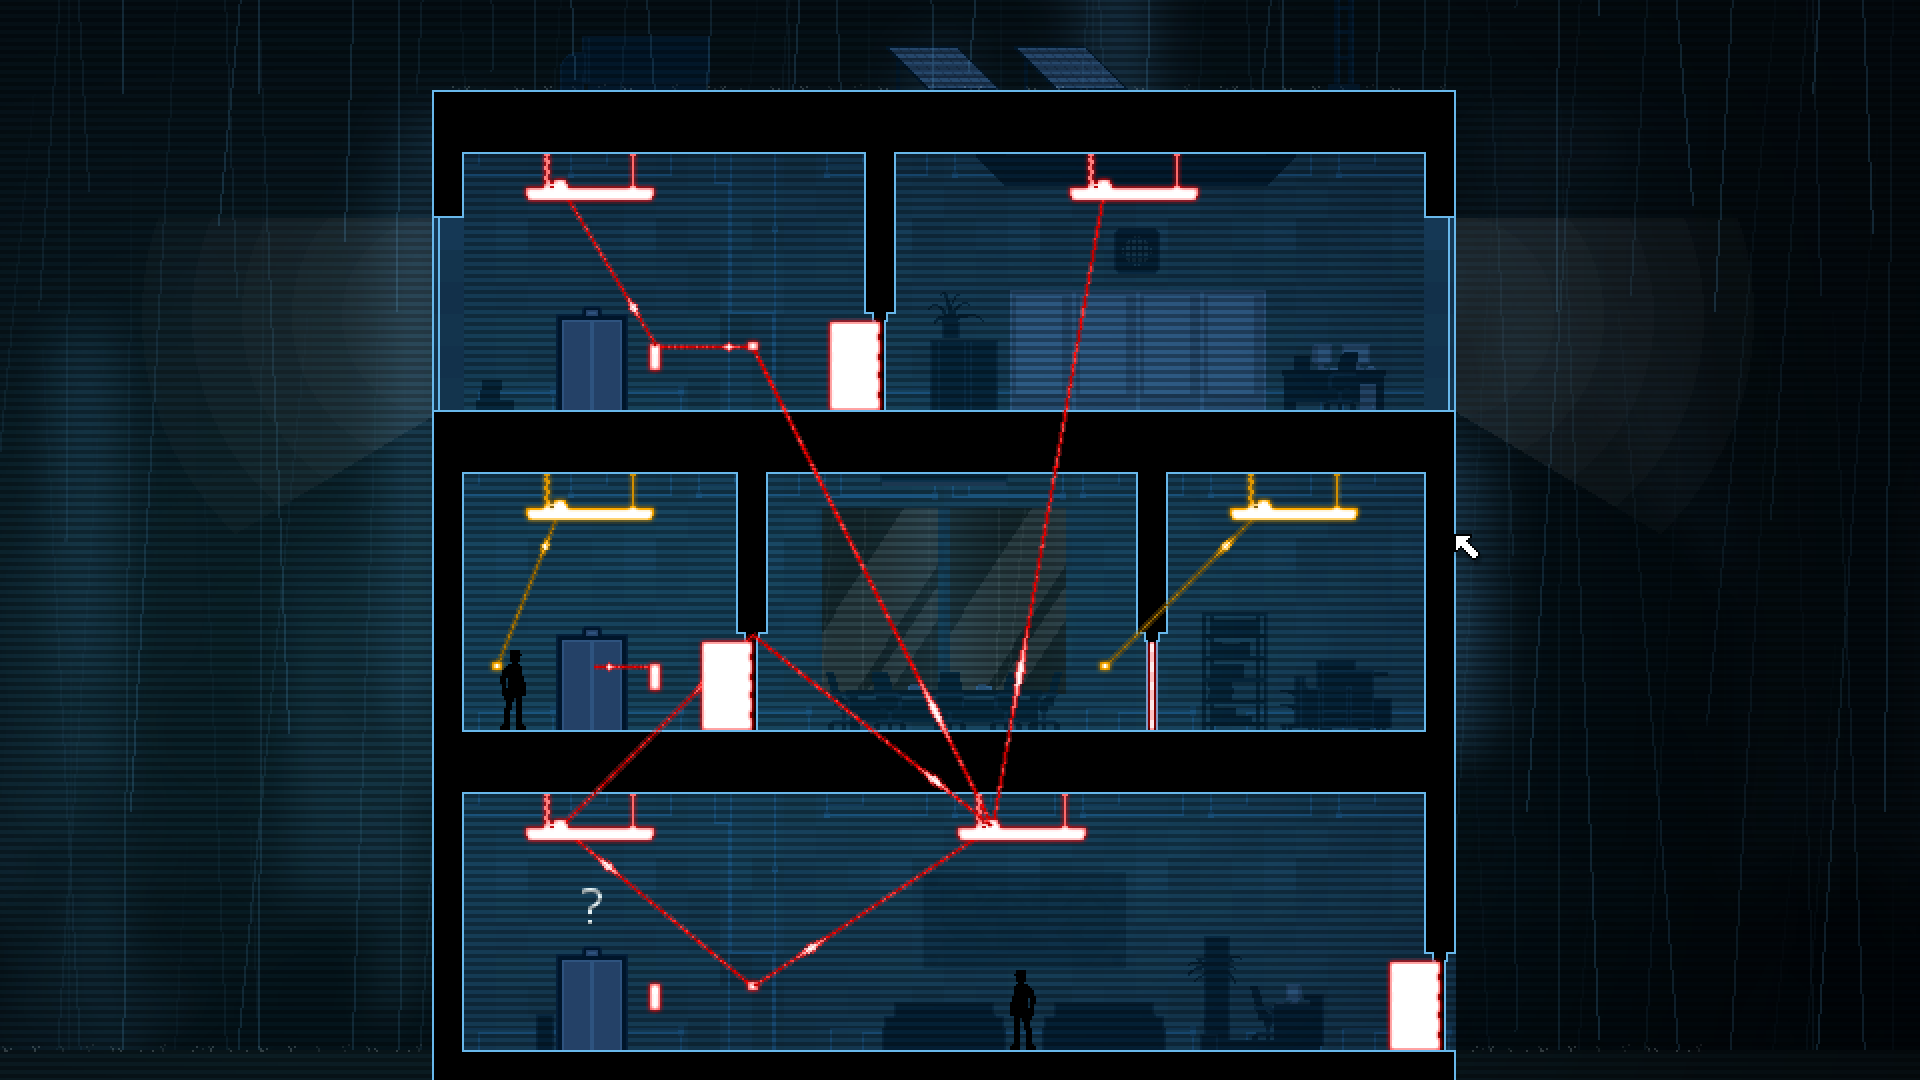
\includegraphics[scale=0.5]{gunpoint}
		\caption{Modo \emph{Crosslink} no jogo Gunpoint}
	\end{figure}

	Dos jogos apresentados, Mark of the Ninja é o mais similar ao jogo proposto, porém Gunpoint oferece uma aproximação diferente para as mecânicas de \emph{stealth}, incluindo elementos \emph{puzzle}. Ambos os jogos foram bem recebidos pela crítica.
	
\end{enumerate}

\AddToShipoutPicture{\BackgroundPic}

\section*{Recursos Tecnológicos Notáveis}
	\begin{figure}[htb]
		\centering
		\includegraphics[scale=0.2]{resources}
		\caption{Logos dos recursos tecnológicos utilizados}
	\end{figure}


%\AddToShipoutPicture{\BackgroundPic}

\section*{Jogos Similares}

\begin{enumerate}
	\item {\Large Mark of the Ninja}
	
	Publicado em 2012 pela Klei Entertainment, também é um jogo de plataforma 2D com elementos \emph{stealth}. O jogador controla um ninja e tem a sua disposição itens como explosivos, shurikens, um gancho, e fogos de artifício para destrair os inimigos. Sons causados tanto pelo jogador quanto pelos inimigos são mostrados na tela como círculos. O jogo possui ambientação moderna. 

	\begin{figure}[htb]
		\centering
		\includegraphics[scale=0.2]{motn}
		\caption{Mark of the Ninja}
	\end{figure}

	\item {\Large Gunpoint}
	
	Publicado em 2013 pelo desenvolvedor independente Tom Francis, Gunpoint não possui muitos elementos tradicionais de plataforma, sendo que maior ênfase é dada a planejamento. A principal mecânica é o chamado Crosslink, que consiste em alterar as conexões elétricas do prédio a ser invadido para abrir caminho (por exemplo, trocar a ligação de um interruptor para que ele abra uma porta ao invés de ligar e desligar uma luz). Essa mecânica também pode ser usada para atacar inimigos (abrir uma porta em cima de um inimigo para desmaiá-lo, por exemplo).

	\begin{figure}[h]
		\centering
		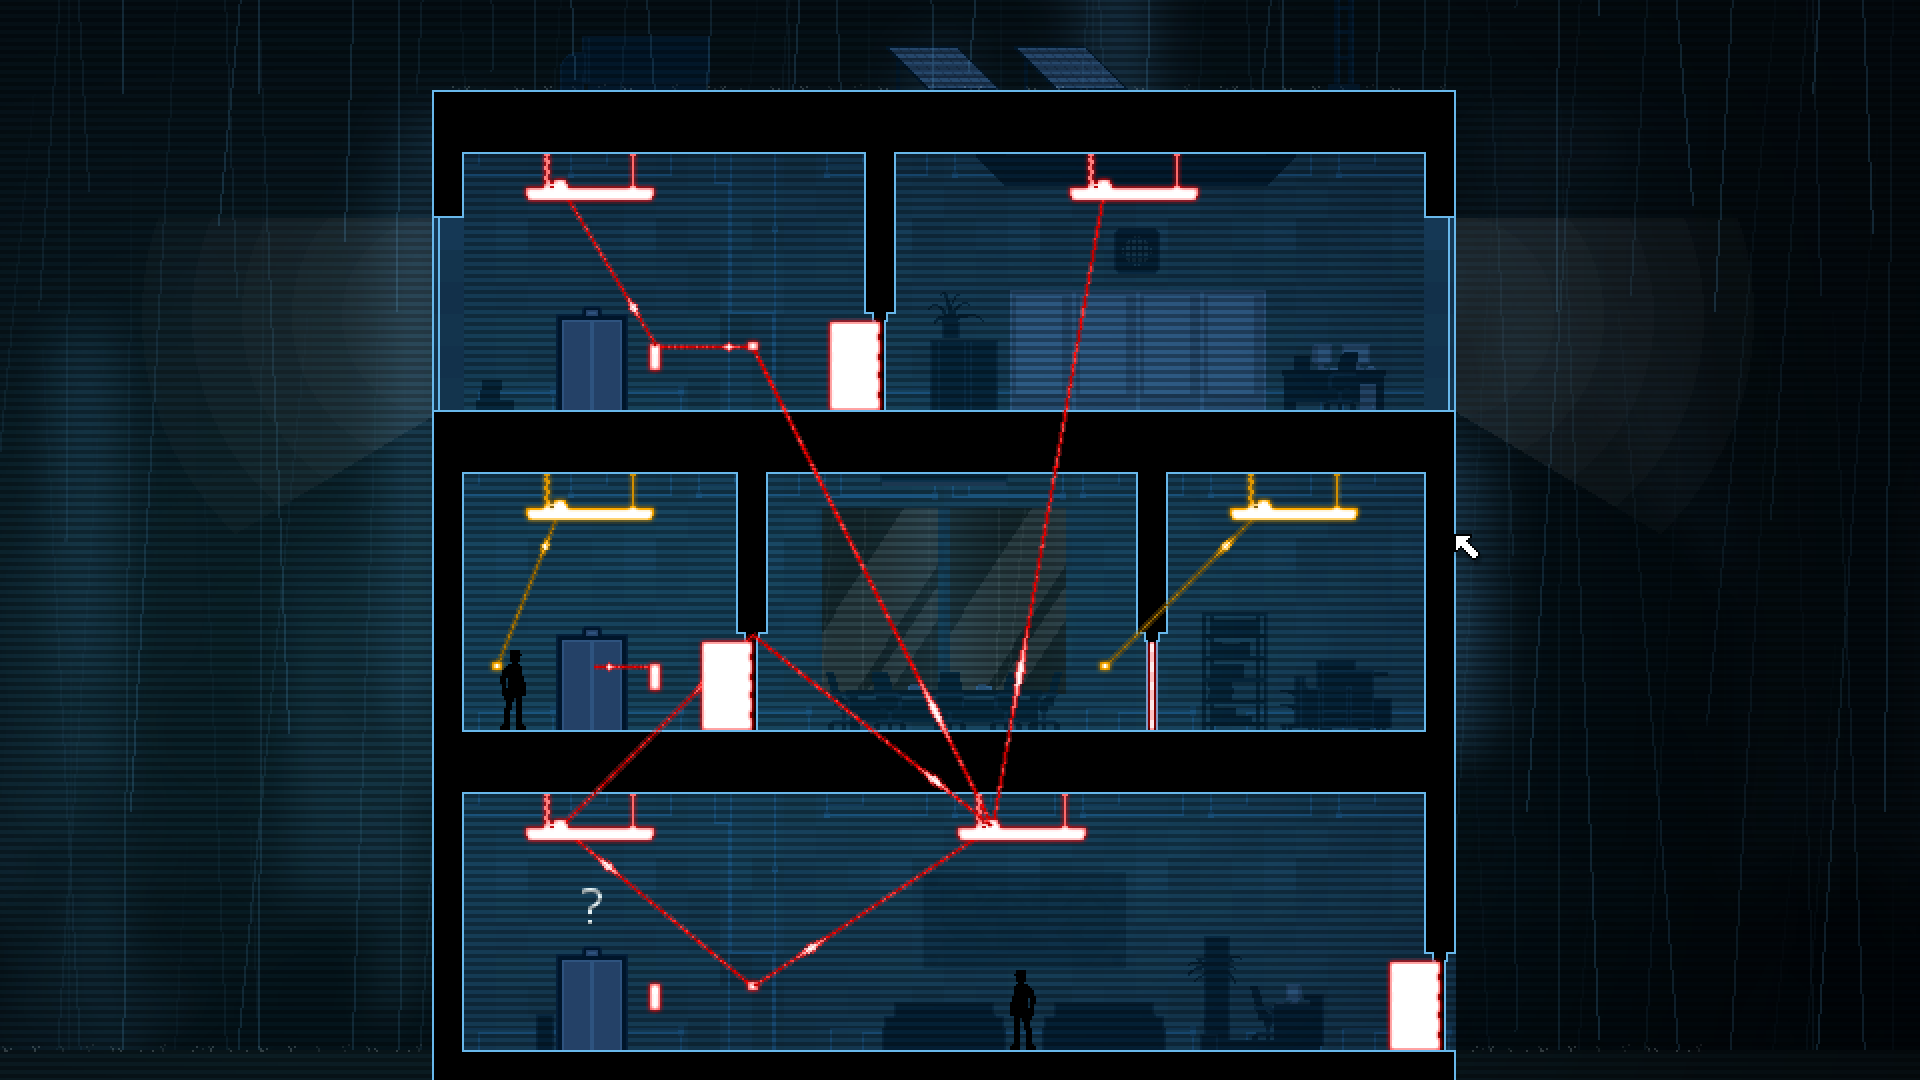
\includegraphics[scale=0.5]{gunpoint}
		\caption{Modo \emph{Crosslink} no jogo Gunpoint}
	\end{figure}

	Dos jogos apresentados, Mark of the Ninja é o mais similar ao jogo proposto, porém Gunpoint oferece uma aproximação diferente para as mecânicas de \emph{stealth}, incluindo elementos \emph{puzzle}. Ambos os jogos foram bem recebidos pela crítica.
	
\end{enumerate}


%\AddToShipoutPicture{\BackgroundPic}

\section*{Recursos Tecnológicos Notáveis}
	\begin{figure}[htb]
		\centering
		\includegraphics[scale=0.2]{resources}
		\caption{Logos dos recursos tecnológicos utilizados}
	\end{figure}


\AddToShipoutPicture{\BackgroundPic}

\section*{Esquema de Controle e Interface com o usuário}

Para controle o jogador utilizará um \emph{joystick} de Playstation 3. As ações mapeadas para cada botão são mostradas na figura~\ref{control}.
 
	\begin{figure}[h]
		\center
		\includegraphics[scale=0.4]{control_scheme.png}
		\caption{Esquema de controle no \emph{joystick}}
		\label{control}
	\end{figure}



\AddToShipoutPicture{\BackgroundPic}

\section*{Relação dos Logotipos}

	\begin{figure}[htb]
		\center
		\includegraphics[scale=0.8]{dauphine_logo}
		\caption{Logo do Jogo}
	\end{figure}
	
	\begin{figure}[htb]
		\center
		\includegraphics[scale=0.5]{alke_logo}
		\caption{Logo do Grupo}
	\end{figure}


\AddToShipoutPicture{\BackgroundPic}
	
	\begin{figure}[htb]
		\vspace{4cm}
		\center
		\includegraphics[scale=0.7]{alke_logo}
	\end{figure}


\end{large}

%\bibliographystyle{ieeetr}
%\bibliography{refs}

\end{document}
